\section{Bauteile}
1mil entspricht $0.0254mm$

Für die meisten Bauteile gilt eine reduktion um $-10K$ eine verdoppelung der Lebensdauer.
\subsection{Widerstände}
\begin{center}
	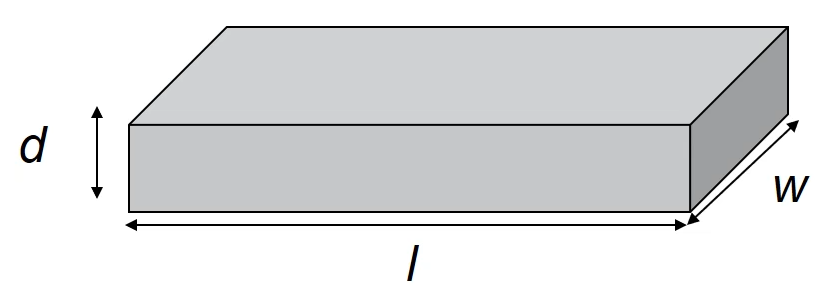
\includegraphics[width=0.4\columnwidth]{Images/widerstand}
\end{center}
\[
R = \rho \frac{l}{w \cdot d}
\]
Für $\rho$ ergeben sich bei Kupfer bei $20^\circ C$ $0.01789\frac{\Omega mm^2}{m}$. Oft ist bei PCB-Herstellern für $d=35\mu m$ gegebene.

\begin{center}
	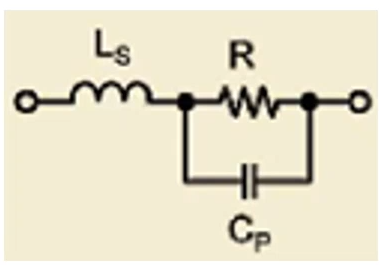
\includegraphics[width=0.3\columnwidth]{Images/widerstand1}
\end{center}
Bei realen Bauteilen ist $L_s$ ca $5nH$ und $C_p$ ca $0.5pF$

\subsection{Kondensatoren}
\begin{center}
	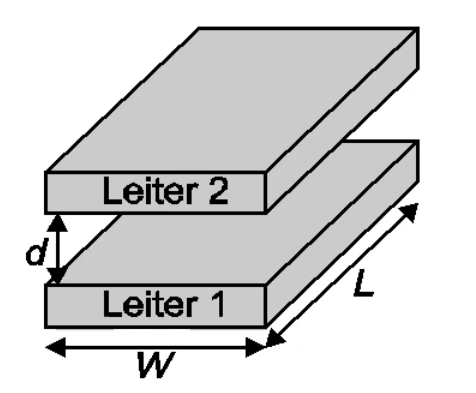
\includegraphics[width=0.3\columnwidth]{Images/kondensator}
\end{center}
\[
C = \frac{W\cdot L}{d}\cdot\varepsilon_r\cdot \varepsilon_0 = \frac{A}{d}\cdot\varepsilon_r\cdot \varepsilon_0
\]
Mit $\varepsilon_0 = 8.85pF/m$, $\varepsilon_r$ entspricht bei Luft $1$ und für FR4 ca. $4.7$

Die \textbf{Ersatzschaltung}, dabei kann Rleak meist vernachlässigt werden.
\begin{center}
	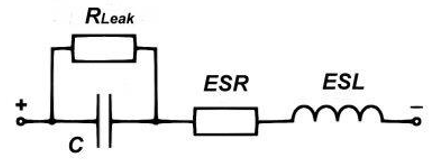
\includegraphics[width=0.6\columnwidth]{Images/kondensator1}
\end{center}


\subsection{Spulen}
\begin{center}
	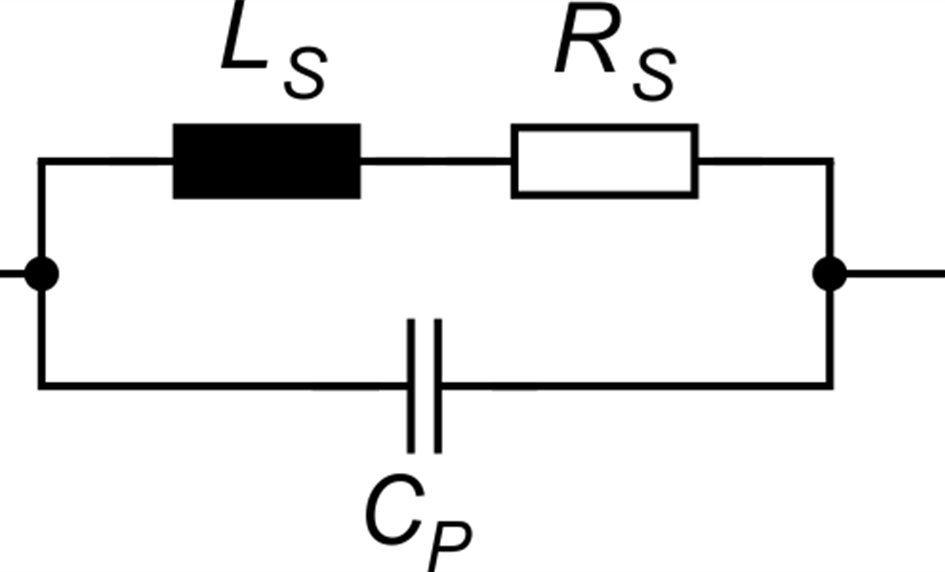
\includegraphics[width=0.6\columnwidth]{Images/spule}
\end{center}
Die Induktivität auf PCB Leiterbahnen kann wie folgt berechnet werden:
\[
L = \frac{\mu l}{\pi}\left(\ln\frac{w}{r}\right)
\]
\begin{center}
	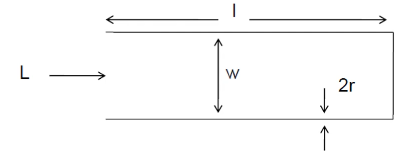
\includegraphics[width=0.6\columnwidth]{Images/spule1}
\end{center}

\subsection{Alterung}
Eine Temperaturerhöhung von 10°C halbiert die Lebensdauer!\\

Für die Reaktionsgeschwindigkeitkonstante gilt:
\[
k = A\cdot e^{-\frac{E_A}{R\cdot T}}
\]
$E_A$ ist die Aktivierungsenergie in $J/mol$. $R = 8.314 j/(K mol)$ die unversale Gaskonstante, $T$ die absolute Temperatu in $K$. Der $A$ Parameter ist der Frequenzfaktor welcher auch Tempeeratur abhängig ist. Als näherung werden oft $A \propto T^n$, wobei oft $n=0.5$ gilt.

Die \textbf{Alterung} von elektronischen Bauteile kann abgeschätzt werden mit:
\[
\lambda_1 = \lambda_0 \cdot e ^{-\frac{E_A}{k}\left(\frac{1}{T}-\frac{1}{T_0}\right)}
\]
Die Ausfallrate $\lambda_0$ bei Ausgangstemperatur $T_0$ kann damit abgeschätzt werden. Die Aktivierungsenergie liegt inder der Regel zwischen $0.1..1.0eV$

\subsection{Thermischer Schaltkreis}
\begin{center}
	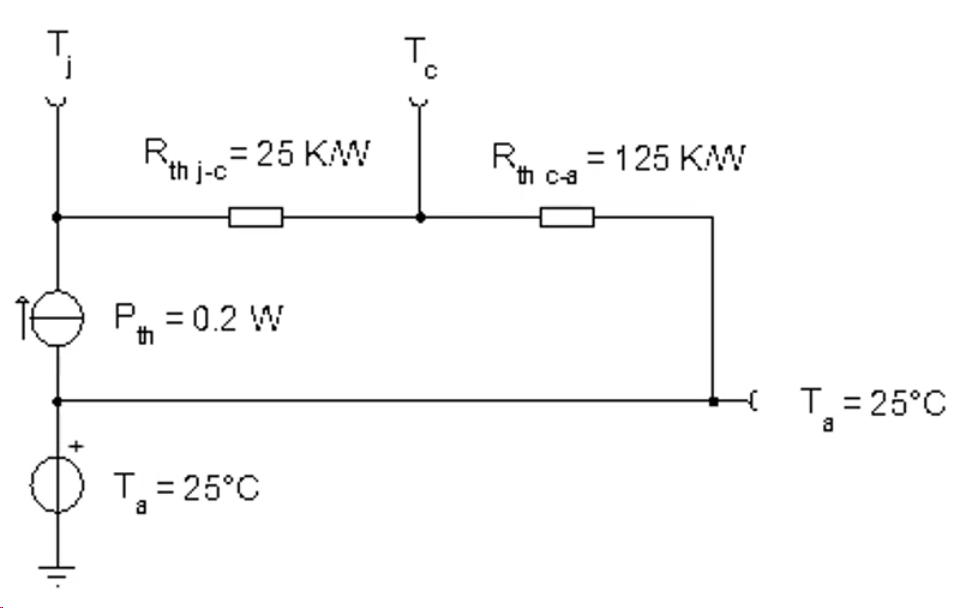
\includegraphics[width=0.6\columnwidth]{Images/thermischerSchaltkreis1}
\end{center}
\begin{align*}
	T_c &= T_a + P_{th}\cdot R_{th c-a} = 25 + 0.2\cdot 125 = 50\\
	T_j &= T_a + P_{th}(R_{th c-a} + R_{th j-c}) = 25 + 0.2(125 + 25) = 55
\end{align*}
Legende
\begin{center}
	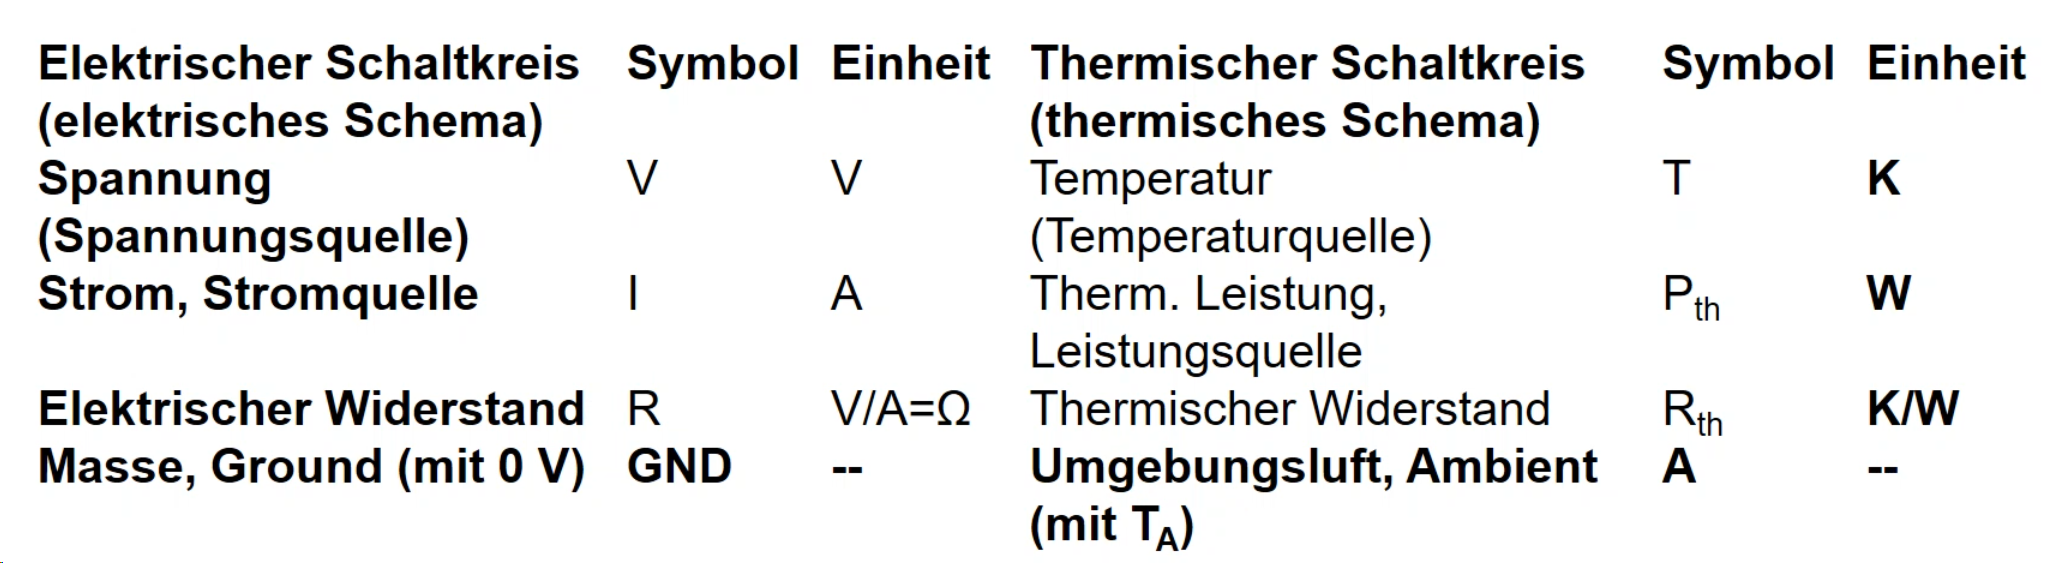
\includegraphics[width=0.8\columnwidth]{Images/thermischerSchaltkreis}
\end{center}
